% SPDX-License-Identifier: GPL-3.0-or-later
\chapter{Obiecte Lansate de Om: Stații Spațiale, Telescoape, Sonde și Rovere}
\label{chap:misiuni}

Începând cu a doua jumătate a secolului XX, omenirea a trimis în cosmos laboratoare orbitale locuite de astronauți, telescoape spațiale plasate deasupra atmosferei terestre, sonde automate care au explorat fiecare planetă a Sistemului Solar și rovere robotice care analizează rocile de pe Marte. În \textbf{Orbitar} sunt modelate 3D și urmărite orbital \textbf{12 misiuni spațiale emblematice}.

\section*{Unde zboară misiunile spațiale? De la Orbita Joasă (LEO) la Punctul Lagrange L2 și Spațiul Interstelar}

\begin{itemize}[leftmargin=1.5em, itemsep=3pt]
  \item \textbf{Orbita Joasă a Pământului (LEO, \emph{Low Earth Orbit}):} situată între $400$ și $600$ de kilometri altitudine deasupra Pământului. Aici zboară \textbf{Stația Spațială Internațională (ISS)} și \textbf{Telescopul Spațial Hubble} cu o viteză orbitală de aproape $28.000$ de kilometri pe oră, înconjurând globul pământesc o dată la fiecare $90\text{--}95\text{ de minute}$. În \textbf{Orbitar}, poziția lor exactă (latitudine, longitudine, altitudine și viteză) este calculată în timp real prin modelul fizic de perturbații \textbf{SGP4} (\texttt{satellite.js}) din elementele orbitale \textbf{NORAD Two-Line Element (TLE)}.
  \item \textbf{Punctul Lagrange L2 Soare--Pământ ($1{,}5\text{ milioane de kilometri}$ de Pământ):} un punct de echilibru gravitațional și centrifugal situat pe linia Soare--Pământ, în spatele Pământului. Aici orbitează \textbf{Telescopul Spațial James Webb (JWST)} și \textbf{Telescopul Spațial Euclid}, astfel încât scuturile lor termice să blocheze simultan căldura Soarelui, a Pământului și a Lunii!
  \item \textbf{Traiectorii interplanetare și interstelare:} sonde precum \textbf{Parker Solar Probe} (care plonjează în coroana Soarelui), \textbf{Rosetta} (care a însoțit cometa 67P), \textbf{JUICE} (în drum spre lunile înghețate ale lui Jupiter), \textbf{New Horizons} (în Centura Kuiper) și gemenele \textbf{Voyager 1 \& 2} (aflate deja în spațiul interstelar!).
  \item \textbf{Suprafața planetei Marte:} roverele nucleare \textbf{Curiosity} (în Craterul Gale) și \textbf{Perseverance \& elicopterul Ingenuity} (în Craterul Jezero), ancorate în \textbf{Orbitar} direct pe coordonatele lor areografice reale de pe globul rotitor al lui Marte.
\end{itemize}

\begin{center}
\begin{tikzpicture}[scale=0.92, every node/.style={transform shape}]
  \fill[orbitarSpaceBg, rounded corners=6pt] (-1.2,-2.2) rectangle (13.4,2.2);
  % Soarele
  \shade[inner color=yellow!95!white, outer color=orange!90!red] (0.4,0) circle (0.85cm);
  \node[white, font=\footnotesize\bfseries] at (0.4,-1.3) {Soarele};

  % Pământul
  \fill[cyan!75!blue] (6.8,0) circle (0.34cm);
  \node[white, font=\footnotesize\bfseries] at (6.8,-0.85) {Pământul (1 UA)};

  % Orbita LEO (ISS & Hubble)
  \draw[orbitarCyan, line width=0.8pt, dashed] (6.8,0) circle (0.58cm);
  \node[orbitarCyan, font=\scriptsize, align=center] at (6.8,1.15) {Orbita LEO ($\sim$420--540 km)\\ISS \& Hubble};

  % Orbita Lunii
  \draw[white!40, line width=0.6pt] (6.8,0) circle (1.45cm);
  \fill[gray!60] (6.8,-1.45) circle (0.11cm);
  \node[white!80, font=\tiny] at (7.8,-1.55) {Luna (384.400 km)};

  % Punctul Lagrange L2
  \draw[orbitarAmber, line width=1.0pt, dashed] (11.2,0) ellipse (0.55cm and 1.1cm);
  \fill[orbitarAmber] (11.2,0) circle (0.10cm);
  \node[amber!90!yellow, font=\footnotesize\bfseries, align=center] at (11.2,1.50) {Punctul Lagrange L2\\JWST \& Euclid};
  \node[white!85, font=\scriptsize, align=center] at (11.2,-1.50) {1,5 mil. km de Pământ\\(Scutul termic spre Soare)};

  \draw[-{Stealth}, white!50, dashed] (1.4,0) -- (6.1,0) node[midway, above, font=\scriptsize, text=white!80] {150 milioane km (1 UA)};
  \draw[-{Stealth}, amber!80, dashed] (7.3,0) -- (10.5,0) node[midway, above, font=\scriptsize, text=amber!80!yellow] {1,5 mil. km};
\end{tikzpicture}
\end{center}

\begin{table}[H]
\centering
\small
\caption{Cele 12 misiuni spațiale (stații, telescoape, sonde și rovere) prezente în Orbitar}
\resizebox{\textwidth}{!}{%
\begin{tabular}{@{}lllrr@{}}
\toprule
\textbf{Misiune / Obiect} & \textbf{Tip} & \textbf{Corp central / Regiune} & \textbf{Distanță Soare} & \textbf{Temp. operare} \\
\midrule
Stația Spațială Internațională (ISS) & Stație Spațială Orbitală & Pământul & 1,00 UA & 21$^\circ$C \\
Telescopul Spațial Hubble & Telescop Spațial & Pământul & 1,00 UA & 15$^\circ$C \\
Telescopul Spațial James Webb (JWST) & Telescop Spațial & Pământul & 1,01 UA & -233$^\circ$C \\
Telescopul Spațial Euclid & Telescop Spațial & Pământul & 1,01 UA & -190$^\circ$C \\
Voyager 1 & Sondă Interplanetară & Soarele (Heliocentric) & 165,00 UA & -195$^\circ$C \\
Voyager 2 & Sondă Interplanetară & Soarele (Heliocentric) & 138,00 UA & -195$^\circ$C \\
New Horizons & Sondă Interplanetară & Soarele (Heliocentric) & 60,20 UA & -210$^\circ$C \\
Parker Solar Probe & Sondă Interplanetară & Soarele (Heliocentric) & 0,25 UA & 1.370$^\circ$C \\
Rosetta \& Philae & Sondă Interplanetară & Soarele (Heliocentric) & 3,46 UA & -70$^\circ$C \\
JUICE (Jupiter Icy Moons Explorer) & Sondă Interplanetară & Soarele (Heliocentric) & 3,10 UA & -150$^\circ$C \\
Perseverance \& Ingenuity & Rover Planetar & Marte & 1,52 UA & -63$^\circ$C \\
Curiosity (Mars Science Laboratory) & Rover Planetar & Marte & 1,52 UA & -63$^\circ$C \\
\bottomrule
\end{tabular}%
}
\end{table}

\begin{tcolorbox}[orbitardata, title={\textbf{Propagare Orbitală SGP4 100\% Offline în Orbitar (\texttt{public/data/tle-iss.json})}}]
Pentru a calcula poziția deasupra continentelor fără a depinde de internet, \textbf{Orbitar} integrează algoritmul astrodinamic \textbf{SGP4} cu seturile oficiale \textbf{NORAD Two-Line Element (TLE)}:
\begin{itemize}[leftmargin=1.4em, itemsep=3pt]
  \item \textbf{ISS (ZARYA), Stația Spațială Internațională (NORAD ID 25544):} altitudine nominală aproximativ 418,5 de kilometri, viteză orbitală aproximativ 27.580 de kilometri pe oră ($15{,}49\text{ orbite/zi}$, înclinație $51{,}64^\circ$).\\
  {\scriptsize\texttt{1 25544U 98067A   24305.51234567  .00016717  00000-0  30124-3 0  9995}}\\
  {\scriptsize\texttt{2 25544  51.6416 247.4627 0006703 130.5360 325.0288 15.49815350479612}}
  \item \textbf{HST, Telescopul Spațial Hubble (NORAD ID 20580):} altitudine nominală aproximativ 535,2 de kilometri, viteză orbitală aproximativ 27.310 de kilometri pe oră ($15{,}12\text{ orbite/zi}$, înclinație $28{,}47^\circ$).\\
  {\scriptsize\texttt{1 20580U 90037B   24305.48123456  .00001842  00000-0  96145-4 0  9991}}\\
  {\scriptsize\texttt{2 20580  28.4698 118.2341 0002640 284.1290  75.9124 15.12498120891245}}
\end{itemize}
\end{tcolorbox}

\begin{tcolorbox}[orbitarjunior, title={\textbf{Discul de Aur Voyager (1977) și Salutul în Limba Română din Spațiul Interstelar}}]
La bordul ambelor sonde \textbf{Voyager 1} și \textbf{Voyager 2} (lansate în august--septembrie 1977) se află \textbf{Discul de Aur (\emph{Voyager Golden Record})}, un disc de cupru placat cu aur cu diametrul de $30$ de centimetri, conceput de o comisie condusă de astronomul \textbf{Carl Sagan} ca o „sticlă cu mesaj în oceanul cosmic”. Discul conține 115 imagini codate analogic, sunete ale naturii terestre, 90 de minute de muzică (Bach, Beethoven, Mozart, folclor mondial) și \textbf{saluturi rostite în 55 de limbi ale Pământului}.\\[4pt]
Printre cele 55 de limbi se află și \textbf{limba română}, cu mesajul rostit de \textbf{Sanda Huffman}:\\
\begin{center}
{\Large\bfseries\color{orbitarDeepBlue}„Salutări la toată lumea!”}
\end{center}
În aplicația \textbf{Orbitar}, când selectezi \emph{Voyager 1} sau \emph{Voyager 2}, poți asculta acest salut istoric direct din caseta dedicată a \textbf{Laboratorului Orbitar}!
\end{tcolorbox}

\begin{tcolorbox}[orbitarcadet, title={\textbf{Atlasul Reperelor Geografice și al Roverelor de pe Marte în Orbitar (\texttt{SurfaceMarkers.ts})}}]
Pe globul 3D al planetei \textbf{Marte}, aplicația \textbf{Orbitar} afișează 6 pini geografici interactivi care marchează rovere active, cratere lacustre fosile și cel mai înalt vulcan din Sistemul Solar:
\begin{enumerate}[leftmargin=1.5em, itemsep=3pt]
  \item \textbf{Roverul Perseverance \& Elicopterul Ingenuity ($18{,}38^\circ\text{ N}, 77{,}58^\circ\text{ E}$, 2021):} laborator astrobiologic mobil de $1.025$ de kilograme amartizat în Craterul Jezero; caută biosemnături străvechi, sigilează tuburi cu mostre de rocă, a produs oxigen pe Marte prin experimentul \emph{MOXIE} și a adus elicopterul \emph{Ingenuity} (care a realizat 72 de zboruri propulsate!).
  \item \textbf{Roverul Curiosity, Mars Science Laboratory ($4{,}58^\circ\text{ S}, 137{,}44^\circ\text{ E}$, 2012):} rover nuclear de $899$ de kilograme care explorează Craterul Gale și urcă pe straturile Muntelui Sharp; a demonstrat că Marte a avut râuri și lacuri cu apă dulce capabile să susțină viața microbiană.
  \item \textbf{Craterul Jezero ($18{,}85^\circ\text{ N}, 77{,}52^\circ\text{ E}$):} crater de impact cu diametrul de $45$ de kilometri care, acum peste $3{,}5\text{ miliarde de ani}$, adăpostea un lac adânc alimentat de un râu, a cărui deltă fluvială fosilă păstrează sedimente de argilă și carbonați.
  \item \textbf{Craterul Gale \& Muntele Sharp / Aeolis Mons ($5{,}4^\circ\text{ S}, 137{,}8^\circ\text{ E}$):} bazin sedimentar cu diametrul de $154$ de kilometri în centrul căruia se înalță \emph{Aeolis Mons} ($5.500$ de metri altitudine), ale cărui straturi de argile și sulfați arată tranziția lui Marte de la o planetă caldă și umedă la un deșert înghețat.
  \item \textbf{Vulcanul Olympus Mons ($18{,}65^\circ\text{ N}, 133{,}8^\circ\text{ V}$):} vulcan-scut gigantic din regiunea Tharsis, cu înălțimea de $21{,}9$ kilometri (de aproape trei ori mai înalt decât Muntele Everest de pe Pământ!) și o bază cu lățimea de $600$ de kilometri, comparabilă cu suprafața României!
  \item \textbf{Chryse Planitia, Sonda Viking 1 ($22{,}27^\circ\text{ N}, 47{,}95^\circ\text{ V}$, 20 iulie 1976):} prima sondă din istorie care a amartizat cu succes și a transmis fotografii color direct de pe solul marțian, funcționând timp de peste 6 ani.
\end{enumerate}
\end{tcolorbox}

\clearpage

\section{Stația Spațială Internațională (ISS)}
\label{sec:body-iss}
\vspace{-4pt}
{\large\itshape\color{orbitarAccent} Laboratorul științific locuit permanent pe orbita joasă a Pământului}\\[4pt]


\begin{center}
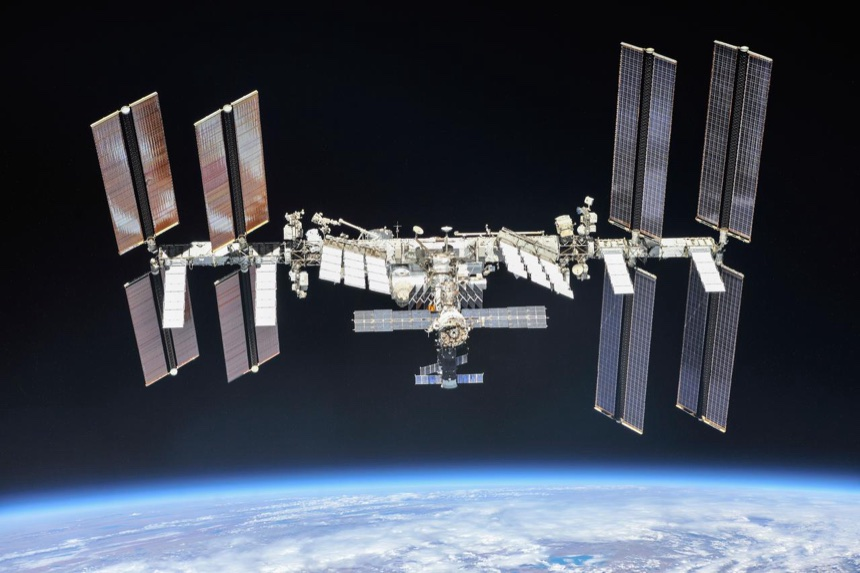
\includegraphics[width=0.78\textwidth,height=5.6cm,keepaspectratio]{../public/textures/nasa/iss.jpg}\\[3pt]
{\footnotesize\itshape\color{orbitarMuted} Fotografie reală NASA (ISS056E201248): Stația Spațială Internațională pe orbita joasă a Pământului (aproximativ 420 de kilometri altitudine).}
\end{center}


\begin{tcolorbox}[orbitardata, title={\textbf{Repere esențiale: Stația Spațială Internațională (ISS)}}]
\small
\begin{itemize}[leftmargin=1.4em, itemsep=2pt, topsep=2pt]
  \item \textbf{Clasificare și orbită:} Stație Spațială Orbitală (orbitează în jurul: \textbf{Pământul}) \quad$\bullet$\quad \textbf{Distanță:} 1,000 UA ($\approx$ 150 milioane de kilometri)
  \item \textbf{Dimensiuni și masă:} anvergură de aproximativ 55 de metri \quad$\bullet$\quad masă: Vehicul spațial artificial
  \item \textbf{Gravitație și regim termic:} Microgravitație / Imponderabilitate ($\approx 0\,g$) \quad$\bullet$\quad temperatură medie: +21 $^\circ$C
  \item \textbf{Ciclu orbital și rotație:} perioadă orbitală (an): 0,064 zile pământești \quad$\bullet$\quad rotație (zi): 1,54 ore (0,06 zile pământești)
  \item \textbf{Durata călătoriei de pe Pământ:} cu viteza luminii ($1c$): \emph{0,0014 secunde}; cu racheta ($50.000$ de kilometri pe oră): \emph{8 minute până pe orbită (și 4--24 ore până la andocare)}; cu avionul ($900$ de kilometri pe oră): \emph{30 de minute (dacă un avion ar putea zbura în sus)}; cu mașina ($100$ de kilometri pe oră): \emph{4 ore pe verticală (se află la aproximativ 410 kilometri altitudine)}.
  \item \textbf{Repere de scară și curiozitate:} ISS este mare cât un teren de fotbal, cu aripi strălucitoare de panouri solare! ISS zboară atât de repede (28.000 kilometri pe oră) încât astronauții văd 16 răsărituri și 16 apusuri de Soare în fiecare zi!
\end{itemize}
\end{tcolorbox}

\vspace{4pt}
\noindent\textbf{Prezentare generală și profil astrofizic.} Construită începând din 1998 prin cooperarea dintre NASA, ESA, Roscosmos, JAXA și CSA, ISS orbitează la aproximativ 410 kilometri altitudine cu o viteză de 7,66 kilometri pe secundă. Este locuită continuu de echipaje umane din noiembrie 2000. Stația Spațială Internațională este o casă și un laborator uriaș care zboară deasupra Pământului! Acolo astronauții plutesc în imponderabilitate și fac experimente pentru toată omenirea. ISS este mare cât un teren de fotbal, cu aripi strălucitoare de panouri solare!

\medskip
\noindent\textbf{Arhitectura tehnică și instrumentele științifice de la bord.} Din punct de vedere constructiv și ingineresc, vehiculul spațial reunește mai multe subsisteme și instrumente științifice de înaltă precizie, proiectate să funcționeze în condițiile extreme ale spațiului cosmic. În primul rând se remarcă \textbf{Module presurizate (Columbus, Destiny, Kibo, Zvezda)}, laboratoare de biologie, fizică a fluidelor, medicină spațială și observații terestre. În strânsă legătură cu această componentă se află \textbf{Grinda centrală (Integrated Truss Structure) și Panourile Solare}, 8 aripi fotovoltaice uriașe care generează peste 120 kW de energie electrică. În completarea acestui ansamblu întâlnim \textbf{Brațul robotic Canadarm2 și Cupola}, braț de manipulare de 17 metri și fereastra panoramică cu 7 geamuri îndreptată spre Pământ.

\medskip
\noindent\textbf{Observații astronomice și istoricul explorării.} Peste 270 de astronauți din peste 20 de țări au lucrat la bordul ISS în mai mult de două decenii de prezență umană neîntreruptă în spațiu. ISS zboară atât de repede (28.000 kilometri pe oră) încât astronauții văd 16 răsărituri și 16 apusuri de Soare în fiecare zi!

\vspace{6pt}
\begin{tcolorbox}[orbitarquiz, title={\textbf{Întrebare de verificare \#35: Stația Spațială Internațională (ISS)}}]
\textbf{În cât timp face Stația Spațială Internațională o tură completă în jurul Pământului?}
\begin{itemize}[leftmargin=2.2em, itemsep=2pt, topsep=4pt]
  \item[$\square$ \textbf{A.}] În 24 de ore
  \item[$\square$ \textbf{B.}] În aproximativ 92 de minute
  \item[$\square$ \textbf{C.}] În 7 zile
  \item[$\square$ \textbf{D.}] Într-o lună
\end{itemize}
\vspace{2pt}
{\footnotesize\color{orbitarMuted}\textbf{Răspuns corect:} \textbf{B} (În aproximativ 92 de minute). \emph{La viteza orbitală de aproximativ 28.000 kilometri pe oră, ISS înconjoară întregul Pământ în aproximativ 92 de minute ( de aproape 16 ori pe zi).}}
\end{tcolorbox}
\clearpage


\section{Telescopul Spațial Hubble}
\label{sec:body-hubble}
\vspace{-4pt}
{\large\itshape\color{orbitarAccent} Ochiul cosmic de pe orbita Pământului care a fotografiat Universul timp de peste 30 de ani}\\[4pt]


\begin{center}
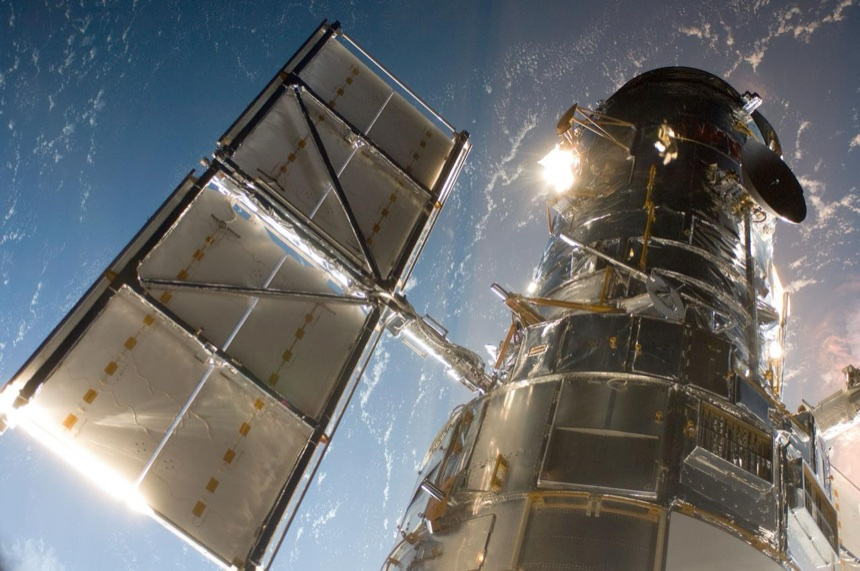
\includegraphics[width=0.78\textwidth,height=5.6cm,keepaspectratio]{../public/textures/nasa/hubble.jpg}\\[3pt]
{\footnotesize\itshape\color{orbitarMuted} Fotografie reală NASA (STS-125): Telescopul Spațial Hubble pe orbită deasupra Pământului.}
\end{center}


\begin{tcolorbox}[orbitardata, title={\textbf{Repere esențiale: Telescopul Spațial Hubble}}]
\small
\begin{itemize}[leftmargin=1.4em, itemsep=2pt, topsep=2pt]
  \item \textbf{Clasificare și orbită:} Telescop Spațial (orbitează în jurul: \textbf{Pământul}) \quad$\bullet$\quad \textbf{Distanță:} 1,000 UA ($\approx$ 150 milioane de kilometri)
  \item \textbf{Dimensiuni și masă:} anvergură de aproximativ 7 metri \quad$\bullet$\quad masă: Vehicul spațial artificial
  \item \textbf{Gravitație și regim termic:} Microgravitație / Imponderabilitate ($\approx 0\,g$) \quad$\bullet$\quad temperatură medie: +15 $^\circ$C
  \item \textbf{Ciclu orbital și rotație:} perioadă orbitală (an): 0,066 zile pământești \quad$\bullet$\quad rotație (zi): 1,58 ore (0,07 zile pământești)
  \item \textbf{Durata călătoriei de pe Pământ:} cu viteza luminii ($1c$): \emph{0,0018 secunde}; cu racheta ($50.000$ de kilometri pe oră): \emph{8 minute și jumătate}; cu avionul ($900$ de kilometri pe oră): \emph{38 de minute}; cu mașina ($100$ de kilometri pe oră): \emph{5 ore și jumătate (540 de kilometri altitudine)}.
  \item \textbf{Repere de scară și curiozitate:} Hubble are mărimea unui autobuz școlar argintiu cu două aripi solare! Hubble are o vedere atât de precisă încât ar putea zări lumina unui licurici aflat la peste 10.000 de kilometri distanță!
\end{itemize}
\end{tcolorbox}

\vspace{4pt}
\noindent\textbf{Prezentare generală și profil astrofizic.} Lansat la 24 aprilie 1990 de naveta Discovery (NASA/ESA), Hubble observă în spectrul vizibil, ultraviolet și infraroșu apropiat de la o altitudine de aproximativ 535 de kilometri, fără distorsiunile atmosferei terestre. Telescopul Hubble este un aparat foto uriaș care plutește în spațiu, deasupra norilor Pământului, și ne trimite cele mai colorate imagini cu nebuloase, stele și galaxii! Hubble are mărimea unui autobuz școlar argintiu cu două aripi solare!

\medskip
\noindent\textbf{Arhitectura tehnică și instrumentele științifice de la bord.} Din punct de vedere constructiv și ingineresc, vehiculul spațial reunește mai multe subsisteme și instrumente științifice de înaltă precizie, proiectate să funcționeze în condițiile extreme ale spațiului cosmic. În primul rând se remarcă \textbf{Oglinda primară Ritchey-Chrétien (2,4 metri diametru)}, șlefuită cu precizie nanometrică și acoperită cu un strat reflectorizant de aluminiu și fluorură de magneziu. În strânsă legătură cu această componentă se află \textbf{Camerele WFC3 și ACS}, instrumente de imagistică cu câmp larg care au realizat celebrele imagini \guillemotleft{}Hubble Ultra-Deep Field\guillemotright{}. În completarea acestui ansamblu întâlnim \textbf{Giroscoape și roți de reacție}, care mențin telescopul îndreptat spre ținte cosmice fără să folosească propulsor chimic care ar murdări oglinda.

\medskip
\noindent\textbf{Observații astronomice și istoricul explorării.} A fost reparat și modernizat direct pe orbită de astronauți în 5 misiuni ale navetelor spațiale (1993--2009), realizând peste 1,6 milioane de observații. Hubble are o vedere atât de precisă încât ar putea zări lumina unui licurici aflat la peste 10.000 de kilometri distanță!

\vspace{6pt}
\begin{tcolorbox}[orbitarquiz, title={\textbf{Întrebare de verificare \#36: Telescopul Spațial Hubble}}]
\textbf{De ce vede Telescopul Hubble mult mai clar decât multe telescoape de pe Pământ?}
\begin{itemize}[leftmargin=2.2em, itemsep=2pt, topsep=4pt]
  \item[$\square$ \textbf{A.}] Pentru că este mult mai aproape de stele
  \item[$\square$ \textbf{B.}] Pentru că se află în spațiu, deasupra atmosferei turbulente a Pământului
  \item[$\square$ \textbf{C.}] Pentru că are o lanternă uriașă
  \item[$\square$ \textbf{D.}] Pentru că se află pe Lună
\end{itemize}
\vspace{2pt}
{\footnotesize\color{orbitarMuted}\textbf{Răspuns corect:} \textbf{B} (Pentru că se află în spațiu, deasupra atmosferei turbulente a Pământului). \emph{Atmosfera Pământului estompează și face stelele să \guillemotleft{}pâlpâie\guillemotright{} (scintilație); aflat în vidul spațial la 535 de kilometri altitudine, Hubble obține imagini de o claritate excepțională.}}
\end{tcolorbox}
\clearpage


\section{Telescopul Spațial James Webb (JWST)}
\label{sec:body-jwst}
\vspace{-4pt}
{\large\itshape\color{orbitarAccent} Cel mai puternic observator spațial în infraroșu, cu oglindă aurită de tip fagure}\\[4pt]


\begin{center}
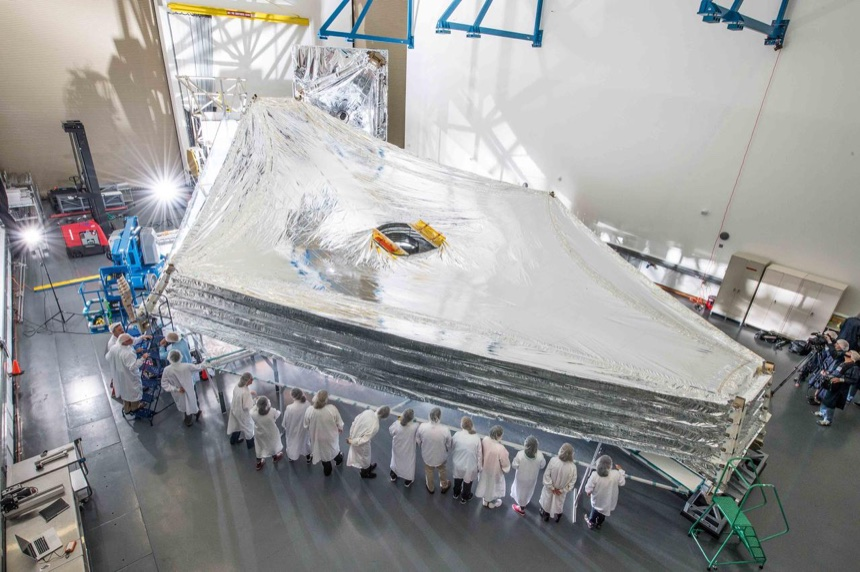
\includegraphics[width=0.78\textwidth,height=5.6cm,keepaspectratio]{../public/textures/nasa/jwst.jpg}\\[3pt]
{\footnotesize\itshape\color{orbitarMuted} Imagine oficială NASA/GSFC: Telescopul Spațial James Webb cu oglinda din 18 segmente hexagonale aurii și scutul termic în 5 straturi.}
\end{center}


\begin{tcolorbox}[orbitardata, title={\textbf{Repere esențiale: Telescopul Spațial James Webb (JWST)}}]
\small
\begin{itemize}[leftmargin=1.4em, itemsep=2pt, topsep=2pt]
  \item \textbf{Clasificare și orbită:} Telescop Spațial (orbitează în jurul: \textbf{Pământul}) \quad$\bullet$\quad \textbf{Distanță:} 1,010 UA ($\approx$ 151 milioane de kilometri)
  \item \textbf{Dimensiuni și masă:} anvergură de aproximativ 11 metri \quad$\bullet$\quad masă: Vehicul spațial artificial
  \item \textbf{Gravitație și regim termic:} Microgravitație / Imponderabilitate ($\approx 0\,g$) \quad$\bullet$\quad temperatură medie: -233 $^\circ$C
  \item \textbf{Ciclu orbital și rotație:} perioadă orbitală (an): 182,62 zile pământești \quad$\bullet$\quad rotație (zi): 24,00 ore (1,00 zile pământești) (elemente kepleriene: $a = 1,010$ UA, $e = 0,0167$, $i = 0,50^\circ$, $\Omega = 0,0^\circ$, $\omega = 102,9^\circ$)
  \item \textbf{Durata călătoriei de pe Pământ:} cu viteza luminii ($1c$): \emph{5 secunde față de Pământ}; cu racheta ($50.000$ de kilometri pe oră): \emph{29 de zile (până în punctul Lagrange L2)}; cu avionul ($900$ de kilometri pe oră): \emph{2 luni și jumătate}; cu mașina ($100$ de kilometri pe oră): \emph{1,7 ani (1,5 milioane de kilometri față de Pământ)}.
  \item \textbf{Repere de scară și curiozitate:} Oglinda lui arată ca un fagure de miere uriaș, iar sub el are o umbrelă de soare cu 5 straturi cât un teren de tenis! Pentru a încăpea în racheta Ariane 5, telescopul a fost împachetat ca un origami și s-a despăturit singur în spațiu!
\end{itemize}
\end{tcolorbox}

\vspace{4pt}
\noindent\textbf{Prezentare generală și profil astrofizic.} Dezvoltat de NASA, ESA și CSA și lansat la 25 decembrie 2021, JWST orbitează în jurul punctului Lagrange L2 Soare--Pământ (la 1,5 milioane de kilometri de Pământ). Observă în infraroșu primele galaxii formate după Big Bang și analizează atmosferele exoplanetelor. Telescopul James Webb este o bijuterie cosmică cu o oglindă mare cât o casă, formată din 18 plăci hexagonale acoperite cu aur adevărat! Oglinda lui arată ca un fagure de miere uriaș, iar sub el are o umbrelă de soare cu 5 straturi cât un teren de tenis!

\medskip
\noindent\textbf{Arhitectura tehnică și instrumentele științifice de la bord.} Din punct de vedere constructiv și ingineresc, vehiculul spațial reunește mai multe subsisteme și instrumente științifice de înaltă precizie, proiectate să funcționeze în condițiile extreme ale spațiului cosmic. În primul rând se remarcă \textbf{Oglinda primară segmentată (6,5 metri diametru)}, 18 segmente hexagonale din beriliu acoperite cu un strat microscopic de aur pentru reflexie maximă în infraroșu. În strânsă legătură cu această componentă se află \textbf{Scutul termic în 5 straturi (Kapton)}, care menține instrumentele la -233 $^\circ$C (40 K), blocând căldura Soarelui, a Pământului și a Lunii. În completarea acestui ansamblu întâlnim \textbf{Instrumentele NIRCam, NIRSpec, MIRI și FGS/NIRISS}, camere și spectrografe capabile să străpungă norii de praf cosmic și să detecteze apă și CO$_2$ pe exoplanete.

\medskip
\noindent\textbf{Observații astronomice și istoricul explorării.} Lansat din Kourou cu o rachetă europeană Ariane 5 în decembrie 2021; a transmis primele imagini științifice revoluționare în iulie 2022. Pentru a încăpea în racheta Ariane 5, telescopul a fost împachetat ca un origami și s-a despăturit singur în spațiu!

\vspace{6pt}
\begin{tcolorbox}[orbitarquiz, title={\textbf{Întrebare de verificare \#37: Telescopul Spațial James Webb (JWST)}}]
\textbf{Din câte segmente hexagonale aurite este alcătuită oglinda principală a Telescopului James Webb?}
\begin{itemize}[leftmargin=2.2em, itemsep=2pt, topsep=4pt]
  \item[$\square$ \textbf{A.}] 6 segmente
  \item[$\square$ \textbf{B.}] 18 segmente
  \item[$\square$ \textbf{C.}] 100 de segmente
  \item[$\square$ \textbf{D.}] Un singur bloc de sticlă
\end{itemize}
\vspace{2pt}
{\footnotesize\color{orbitarMuted}\textbf{Răspuns corect:} \textbf{B} (18 segmente). \emph{Oglinda de 6,5 metri a JWST este formată din 18 segmente hexagonale din beriliu aurit care s-au depliat și aliniat la nivel nanometric în spațiu.}}
\end{tcolorbox}
\clearpage


\section{Telescopul Spațial Euclid}
\label{sec:body-euclid}
\vspace{-4pt}
{\large\itshape\color{orbitarAccent} Cartograful european al Universului Întunecat (în punctul Lagrange L2)}\\[4pt]


\begin{center}
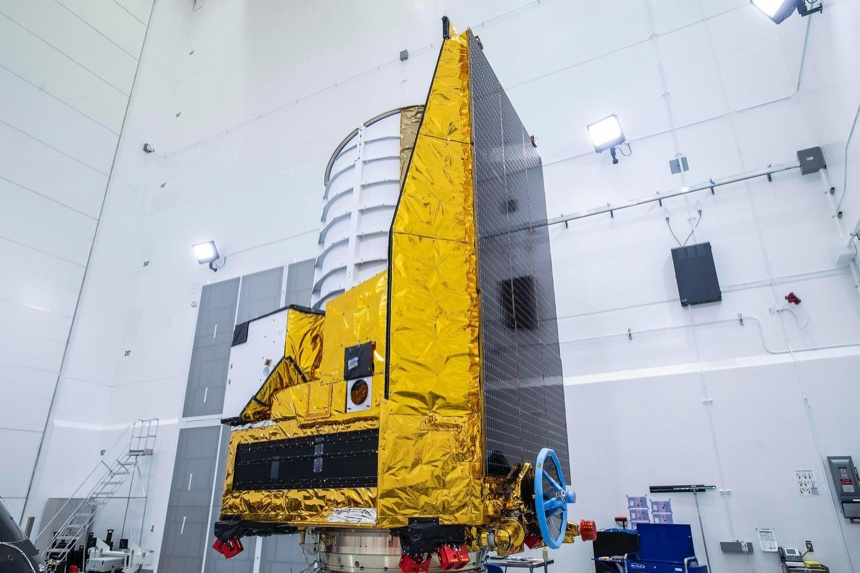
\includegraphics[width=0.78\textwidth,height=5.6cm,keepaspectratio]{../public/textures/nasa/euclid.jpg}\\[3pt]
{\footnotesize\itshape\color{orbitarMuted} Fotografie oficială NASA/ESA (PIA25783): Telescopul Spațial Euclid pentru cartografierea materiei și energiei întunecate.}
\end{center}


\begin{tcolorbox}[orbitardata, title={\textbf{Repere esențiale: Telescopul Spațial Euclid}}]
\small
\begin{itemize}[leftmargin=1.4em, itemsep=2pt, topsep=2pt]
  \item \textbf{Clasificare și orbită:} Telescop Spațial (orbitează în jurul: \textbf{Pământul}) \quad$\bullet$\quad \textbf{Distanță:} 1,010 UA ($\approx$ 151 milioane de kilometri)
  \item \textbf{Dimensiuni și masă:} anvergură de aproximativ 2 metri \quad$\bullet$\quad masă: Vehicul spațial artificial
  \item \textbf{Gravitație și regim termic:} Microgravitație / Imponderabilitate ($\approx 0\,g$) \quad$\bullet$\quad temperatură medie: -190 $^\circ$C
  \item \textbf{Ciclu orbital și rotație:} perioadă orbitală (an): 182,62 zile pământești \quad$\bullet$\quad rotație (zi): 24,00 ore (1,00 zile pământești) (elemente kepleriene: $a = 1,010$ UA, $e = 0,0180$, $i = 1,20^\circ$, $\Omega = 18,0^\circ$, $\omega = 98,0^\circ$)
  \item \textbf{Durata călătoriei de pe Pământ:} cu viteza luminii ($1c$): \emph{5 secunde față de Pământ}; cu racheta ($50.000$ de kilometri pe oră): \emph{30 de zile până în L2}; cu avionul ($900$ de kilometri pe oră): \emph{2 luni și jumătate}; cu mașina ($100$ de kilometri pe oră): \emph{1,7 ani (1,5 milioane de kilometri de Pământ)}.
  \item \textbf{Repere de scară și curiozitate:} Dacă James Webb este o lupă super-puternică ce privește un singur detaliu, Euclid este un aparat foto panoramic care cuprinde o bucată uriașă de cer dintr-odată! Numele lui vine de la Euclid din Alexandria, matematicianul antic numit \guillemotleft{}părintele geometriei\guillemotright{}!
\end{itemize}
\end{tcolorbox}

\vspace{4pt}
\noindent\textbf{Prezentare generală și profil astrofizic.} Lansat în iulie 2023 de ESA, Euclid operează în punctul Lagrange L2 pentru a investiga natura materiei întunecate și a energiei întunecate, cartografiind distribuția tridimensională a miliarde de galaxii pe o distanță de 10 miliarde de ani-lumină. Euclid este telescopul Agenției Spațiale Europene (ESA) trimis să deseneze cea mai mare hartă 3D a miliarde de galaxii din Univers! Dacă James Webb este o lupă super-puternică ce privește un singur detaliu, Euclid este un aparat foto panoramic care cuprinde o bucată uriașă de cer dintr-odată!

\medskip
\noindent\textbf{Arhitectura tehnică și instrumentele științifice de la bord.} Din punct de vedere constructiv și ingineresc, vehiculul spațial reunește mai multe subsisteme și instrumente științifice de înaltă precizie, proiectate să funcționeze în condițiile extreme ale spațiului cosmic. În primul rând se remarcă \textbf{Telescop Korsch din carbură de siliciu (1,2 metri)}, material ceramic ultra-stabil termic care previne orice deformare optică. În strânsă legătură cu această componentă se află \textbf{Camera în spectru vizibil VIS (600 megapixeli)}, care măsoară cu precizie extremă forma galaxiilor și efectul de lentilă gravitațională slabă. În completarea acestui ansamblu întâlnim \textbf{Spectrometrul și fotometrul în infraroșu apropiat NISP}, care determină distanța (redshift-ul) fiecărei galaxii observate.

\medskip
\noindent\textbf{Observații astronomice și istoricul explorării.} Lansat la 1 iulie 2023; primele sale imagini cosmice (\guillemotleft{}Early Release Observations\guillemotright{}) au dezvăluit roiul Perseus și mii de galaxii necunoscute anterior. Numele lui vine de la Euclid din Alexandria, matematicianul antic numit \guillemotleft{}părintele geometriei\guillemotright{}!

\vspace{6pt}
\begin{tcolorbox}[orbitarquiz, title={\textbf{Întrebare de verificare \#38: Telescopul Spațial Euclid}}]
\textbf{Care este obiectivul științific principal al misiunii europene Euclid?}
\begin{itemize}[leftmargin=2.2em, itemsep=2pt, topsep=4pt]
  \item[$\square$ \textbf{A.}] Asolizarea pe Venus
  \item[$\square$ \textbf{B.}] Realizarea unei hărți 3D a miliarde de galaxii pentru a studia materia și energia întunecată
  \item[$\square$ \textbf{C.}] Fotografierea petelor solare
  \item[$\square$ \textbf{D.}] Colectarea de roci lunare
\end{itemize}
\vspace{2pt}
{\footnotesize\color{orbitarMuted}\textbf{Răspuns corect:} \textbf{B} (Realizarea unei hărți 3D a miliarde de galaxii pentru a studia materia și energia întunecată). \emph{Euclid măsoară geometria la scară mare a Universului pentru a înțelege cum materia întunecată și energia întunecată îi modelează expansiunea.}}
\end{tcolorbox}
\clearpage


\section{Voyager 1}
\label{sec:body-voyager1}
\vspace{-4pt}
{\large\itshape\color{orbitarAccent} Cel mai îndepărtat obiect creat de om, călătorind în spațiul interstelar}\\[4pt]


\begin{center}
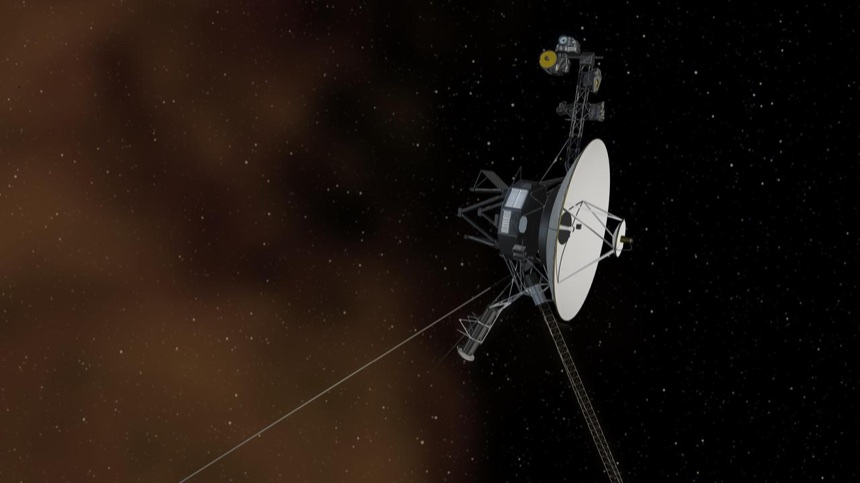
\includegraphics[width=0.78\textwidth,height=5.6cm,keepaspectratio]{../public/textures/nasa/voyager1.jpg}\\[3pt]
{\footnotesize\itshape\color{orbitarMuted} Randare oficială NASA/JPL-Caltech (PIA17462): Sonda Voyager 1 călătorind în spațiul interstelar cu Discul de Aur la bord.}
\end{center}


\begin{tcolorbox}[orbitardata, title={\textbf{Repere esențiale: Voyager 1}}]
\small
\begin{itemize}[leftmargin=1.4em, itemsep=2pt, topsep=2pt]
  \item \textbf{Clasificare și orbită:} Sondă Interplanetară \quad$\bullet$\quad \textbf{Distanță:} 165,000 UA ($\approx$ 24.684 milioane de kilometri)
  \item \textbf{Dimensiuni și masă:} anvergură de aproximativ 2 metri \quad$\bullet$\quad masă: Vehicul spațial artificial
  \item \textbf{Gravitație și regim termic:} Microgravitație / Imponderabilitate ($\approx 0\,g$) \quad$\bullet$\quad temperatură medie: -195 $^\circ$C
  \item \textbf{Ciclu orbital și rotație:} perioadă orbitală (an): 180.000 zile ($\approx$ 492,81 ani pământești) \quad$\bullet$\quad rotație (zi): 24,00 ore (1,00 zile pământești) (elemente kepleriene: $a = 42,500$ UA, $e = 0,2500$, $i = 35,70^\circ$, $\Omega = 178,0^\circ$, $\omega = 85,0^\circ$)
  \item \textbf{Durata călătoriei de pe Pământ:} cu viteza luminii ($1c$): \emph{22 de ore și 45 de minute}; cu racheta ($50.000$ de kilometri pe oră): \emph{47+ ani de zbor continuu (cu 61.000 kilometri pe oră)}; cu avionul ($900$ de kilometri pe oră): \emph{3.100 de ani}; cu mașina ($100$ de kilometri pe oră): \emph{28.000 de ani}.
  \item \textbf{Repere de scară și curiozitate:} Poartă cu ea un \guillemotleft{}Disc de Aur\guillemotright{} cu saluturi în 55 de limbi (inclusiv în limba română: \guillemotleft{}Salutări la toată lumea!\guillemotright{}), muzică și sunete de pe Pământ! Voyager 1 este atât de departe încât un mesaj radio care merge cu viteza luminii face aproape o zi întreagă până ajunge la ea!
\end{itemize}
\end{tcolorbox}

\vspace{4pt}
\noindent\textbf{Prezentare generală și profil astrofizic.} Lansată la 5 septembrie 1977, Voyager 1 a explorat sistemele lui Jupiter (1979) și Saturn (1980), iar la 25 august 2012 a traversat heliopauza, devenind primul artefact uman care pătrunde în mediul interstelar, la peste 24 de miliarde de kilometri de Pământ. Voyager 1 este cel mai curajos explorator construit vreodată de oameni! Zboară din anul 1977 și a ieșit deja din Sistemul Solar, în spațiul dintre stele. Poartă cu ea un \guillemotleft{}Disc de Aur\guillemotright{} cu saluturi în 55 de limbi (inclusiv în limba română: \guillemotleft{}Salutări la toată lumea!\guillemotright{}), muzică și sunete de pe Pământ!

\medskip
\noindent\textbf{Arhitectura tehnică și instrumentele științifice de la bord.} Din punct de vedere constructiv și ingineresc, vehiculul spațial reunește mai multe subsisteme și instrumente științifice de înaltă precizie, proiectate să funcționeze în condițiile extreme ale spațiului cosmic. În primul rând se remarcă \textbf{Antena parabolică de mare câștig (3,7 metri diametru)}, menținută permanent orientată către Pământ pentru comunicații prin rețeaua Deep Space Network. În strânsă legătură cu această componentă se află \textbf{Generatoare termoelectrice cu radioizotopi (3 $\times$ RTG)}, alimentate cu plutoniu-238, deoarece la distanțe mari lumina Soarelui este prea slabă pentru panouri solare. În completarea acestui ansamblu întâlnim \textbf{Discul de Aur (Voyager Golden Record) și Magnetometrele}, capsulă culturală a umanității și senzori care măsoară plasma și câmpul magnetic interstelar.

\medskip
\noindent\textbf{Observații astronomice și istoricul explorării.} A realizat în 1990 celebra fotografie a Pământului \guillemotleft{}Un punct albastru pal\guillemotright{} (Pale Blue Dot) de la 6 miliarde de kilometri distanță, la sugestia lui Carl Sagan. Voyager 1 este atât de departe încât un mesaj radio care merge cu viteza luminii face aproape o zi întreagă până ajunge la ea!

\vspace{6pt}
\begin{tcolorbox}[orbitarquiz, title={\textbf{Întrebare de verificare \#39: Voyager 1}}]
\textbf{Ce poartă la bord sondele Voyager 1 și Voyager 2 ca mesaj pentru eventuale civilizații extraterestre?}
\begin{itemize}[leftmargin=2.2em, itemsep=2pt, topsep=4pt]
  \item[$\square$ \textbf{A.}] Discul de Aur (Golden Record) cu sunete, imagini și saluturi în 55 de limbi, inclusiv în română
  \item[$\square$ \textbf{B.}] Un steag de hârtie
  \item[$\square$ \textbf{C.}] Un telescop cu oglindă de aur
  \item[$\square$ \textbf{D.}] Roci de pe Lună
\end{itemize}
\vspace{2pt}
{\footnotesize\color{orbitarMuted}\textbf{Răspuns corect:} \textbf{A} (Discul de Aur (Golden Record) cu sunete, imagini și saluturi în 55 de limbi, inclusiv în română). \emph{Discul de Aur Voyager conține 115 imagini, muzică de pe Pământ și saluturi în 55 de limbi (inclusiv \guillemotleft{}Salutări la toată lumea\guillemotright{} în limba română).}}
\end{tcolorbox}
\clearpage


\section{Voyager 2}
\label{sec:body-voyager2}
\vspace{-4pt}
{\large\itshape\color{orbitarAccent} Singura sondă din istorie care a vizitat toți cei 4 giganți: Jupiter, Saturn, Uranus și Neptun}\\[4pt]


\begin{center}
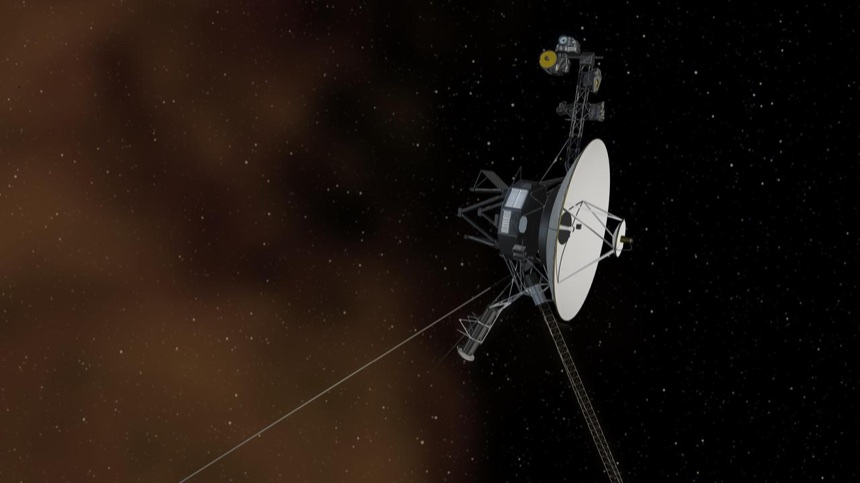
\includegraphics[width=0.78\textwidth,height=5.6cm,keepaspectratio]{../public/textures/nasa/voyager2.jpg}\\[3pt]
{\footnotesize\itshape\color{orbitarMuted} Randare oficială NASA/JPL-Caltech (PIA17462): Sonda Voyager 2, singura navă care a vizitat toți cei patru giganți planetari.}
\end{center}


\begin{tcolorbox}[orbitardata, title={\textbf{Repere esențiale: Voyager 2}}]
\small
\begin{itemize}[leftmargin=1.4em, itemsep=2pt, topsep=2pt]
  \item \textbf{Clasificare și orbită:} Sondă Interplanetară \quad$\bullet$\quad \textbf{Distanță:} 138,000 UA ($\approx$ 20.645 milioane de kilometri)
  \item \textbf{Dimensiuni și masă:} anvergură de aproximativ 2 metri \quad$\bullet$\quad masă: Vehicul spațial artificial
  \item \textbf{Gravitație și regim termic:} Microgravitație / Imponderabilitate ($\approx 0\,g$) \quad$\bullet$\quad temperatură medie: -195 $^\circ$C
  \item \textbf{Ciclu orbital și rotație:} perioadă orbitală (an): 165.000 zile ($\approx$ 451,75 ani pământești) \quad$\bullet$\quad rotație (zi): 24,00 ore (1,00 zile pământești) (elemente kepleriene: $a = 38,500$ UA, $e = 0,2200$, $i = -32,00^\circ$, $\Omega = 310,0^\circ$, $\omega = 45,0^\circ$)
  \item \textbf{Durata călătoriei de pe Pământ:} cu viteza luminii ($1c$): \emph{19 ore}; cu racheta ($50.000$ de kilometri pe oră): \emph{47+ ani}; cu avionul ($900$ de kilometri pe oră): \emph{2.600 de ani}; cu mașina ($100$ de kilometri pe oră): \emph{23.500 de ani}.
  \item \textbf{Repere de scară și curiozitate:} Folosind gravitația fiecărei planete ca pe o praștie cosmică, Voyager 2 a sărit de la o planetă la alta! Deși se numește Voyager 2, a fost lansată cu 16 zile ÎNAINTE de Voyager 1!
\end{itemize}
\end{tcolorbox}

\vspace{4pt}
\noindent\textbf{Prezentare generală și profil astrofizic.} Lansată la 20 august 1977, Voyager 2 a profitat de o aliniere planetară care apare doar o dată la 175 de ani (\guillemotleft{}Grand Tour\guillemotright{}), survolând Jupiter (1979), Saturn (1981), Uranus (1986) și Neptun (1989). În noiembrie 2018 a intrat și ea în spațiul interstelar. Voyager 2 este sora geamănă a lui Voyager 1 și singura navă spațială care a făcut \guillemotleft{}Marele Tur\guillemotright{}, vizitând toate cele patru planete uriașe: Jupiter, Saturn, Uranus și Neptun! Folosind gravitația fiecărei planete ca pe o praștie cosmică, Voyager 2 a sărit de la o planetă la alta!

\medskip
\noindent\textbf{Arhitectura tehnică și instrumentele științifice de la bord.} Din punct de vedere constructiv și ingineresc, vehiculul spațial reunește mai multe subsisteme și instrumente științifice de înaltă precizie, proiectate să funcționeze în condițiile extreme ale spațiului cosmic. În primul rând se remarcă \textbf{Antena parabolică de 3,7 metri și emițătorul în banda X}, prin care transmite date științifice cu o putere de doar aproximativ 20 W (cât un bec de frigider) de la peste 20 de miliarde de kilometri. În strânsă legătură cu această componentă se află \textbf{Sub-sistemul de analiză a plasmei (PLS)}, care a măsurat direct tranziția bruscă de la vântul solar cald la plasma interstelară rece. În completarea acestui ansamblu întâlnim \textbf{Platforma de scanare cu camere și spectrometre}, care a descoperit 16 sateliți noi, gheizerele de azot de pe Triton și inelele lui Uranus și Neptun.

\medskip
\noindent\textbf{Observații astronomice și istoricul explorării.} Rămâne până astăzi singura sondă care a explorat de aproape giganții de gheață Uranus și Neptun. Deși se numește Voyager 2, a fost lansată cu 16 zile ÎNAINTE de Voyager 1!

\vspace{6pt}
\begin{tcolorbox}[orbitarquiz, title={\textbf{Întrebare de verificare \#40: Voyager 2}}]
\textbf{Care este singura sondă spațială care a vizitat planetele Uranus și Neptun?}
\begin{itemize}[leftmargin=2.2em, itemsep=2pt, topsep=4pt]
  \item[$\square$ \textbf{A.}] Voyager 1
  \item[$\square$ \textbf{B.}] Voyager 2
  \item[$\square$ \textbf{C.}] Cassini
  \item[$\square$ \textbf{D.}] New Horizons
\end{itemize}
\vspace{2pt}
{\footnotesize\color{orbitarMuted}\textbf{Răspuns corect:} \textbf{B} (Voyager 2). \emph{Voyager 2 este singura navă spațială care a survolat toate cele patru planete gigante, inclusiv Uranus (1986) și Neptun (1989).}}
\end{tcolorbox}
\clearpage


\section{New Horizons}
\label{sec:body-newhorizons}
\vspace{-4pt}
{\large\itshape\color{orbitarAccent} Sonda rapidă care ne-a dezvăluit inima înghețată a lui Pluto și Centura Kuiper}\\[4pt]


\begin{center}
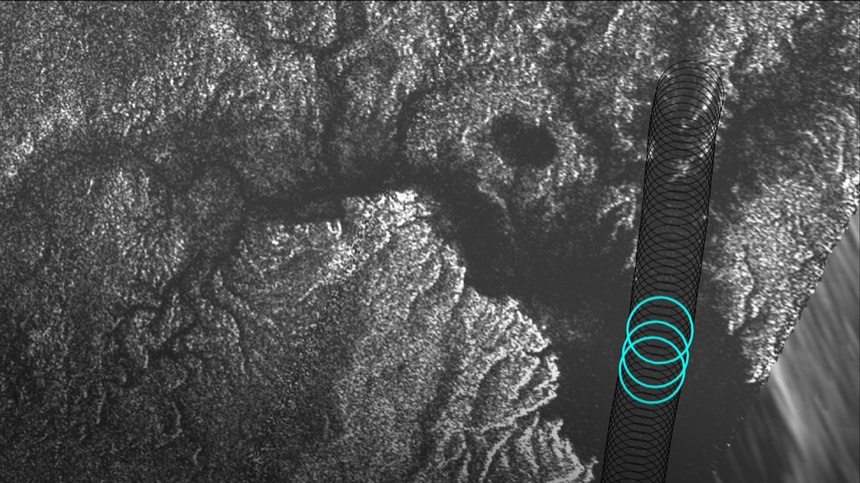
\includegraphics[width=0.78\textwidth,height=5.6cm,keepaspectratio]{../public/textures/nasa/newhorizons.jpg}\\[3pt]
{\footnotesize\itshape\color{orbitarMuted} Imagine oficială NASA/JHUAPL/SwRI: Sonda interplanetară New Horizons în timpul explorării Centurii Kuiper.}
\end{center}


\begin{tcolorbox}[orbitardata, title={\textbf{Repere esențiale: New Horizons}}]
\small
\begin{itemize}[leftmargin=1.4em, itemsep=2pt, topsep=2pt]
  \item \textbf{Clasificare și orbită:} Sondă Interplanetară \quad$\bullet$\quad \textbf{Distanță:} 60,200 UA ($\approx$ 9.006 milioane de kilometri)
  \item \textbf{Dimensiuni și masă:} anvergură de aproximativ 2,1 metri \quad$\bullet$\quad masă: Vehicul spațial artificial
  \item \textbf{Gravitație și regim termic:} Microgravitație / Imponderabilitate ($\approx 0\,g$) \quad$\bullet$\quad temperatură medie: -210 $^\circ$C
  \item \textbf{Ciclu orbital și rotație:} perioadă orbitală (an): 120.000 zile ($\approx$ 328,54 ani pământești) \quad$\bullet$\quad rotație (zi): 24,00 ore (1,00 zile pământești) (elemente kepleriene: $a = 35,000$ UA, $e = 0,2800$, $i = 14,50^\circ$, $\Omega = 115,0^\circ$, $\omega = 180,0^\circ$)
  \item \textbf{Durata călătoriei de pe Pământ:} cu viteza luminii ($1c$): \emph{8 ore și 20 de minute}; cu racheta ($50.000$ de kilometri pe oră): \emph{9,5 ani până la Pluto (18+ ani în Centura Kuiper)}; cu avionul ($900$ de kilometri pe oră): \emph{1.100 de ani}; cu mașina ($100$ de kilometri pe oră): \emph{10.000 de ani}.
  \item \textbf{Repere de scară și curiozitate:} A plecat de pe Pământ mai repede decât orice altă rachetă și a trecut de orbita Lunii în doar 9 ore (față de 3 zile cât le-a luat astronauților Apollo)! După Pluto, a vizitat în 2019 și pe Arrokoth, un corp înghețat din Centura Kuiper care arată exact ca un om de zăpadă cosmic!
\end{itemize}
\end{tcolorbox}

\vspace{4pt}
\noindent\textbf{Prezentare generală și profil astrofizic.} Lansată la 19 ianuarie 2006 cu cea mai mare viteză de evadare de pe Pământ (16,26 kilometri pe secundă), New Horizons a survolat Jupiter în 2007, sistemul Pluto--Charon la 14 iulie 2015 și obiectul primordial din Centura Kuiper 486958 Arrokoth la 1 ianuarie 2019. New Horizons este sonda spațială de mărimea unui pian cu coadă care a zburat timp de 9 ani și jumătate pentru a fotografia pentru prima oară de aproape planeta pitică Pluto! A plecat de pe Pământ mai repede decât orice altă rachetă și a trecut de orbita Lunii în doar 9 ore (față de 3 zile cât le-a luat astronauților Apollo)!

\medskip
\noindent\textbf{Arhitectura tehnică și instrumentele științifice de la bord.} Din punct de vedere constructiv și ingineresc, vehiculul spațial reunește mai multe subsisteme și instrumente științifice de înaltă precizie, proiectate să funcționeze în condițiile extreme ale spațiului cosmic. În primul rând se remarcă \textbf{Camera telescopică LORRI și spectrometrul Ralph}, care au cartografiat munții de gheață și câmpia Sputnik Planitia de pe Pluto la rezoluții de sub 100 de metri pe pixel. În strânsă legătură cu această componentă se află \textbf{Generator radioizotopic RTG și antenă de 2,1 metri}, care asigură energia și comunicațiile la peste 55--60 UA de Soare. În completarea acestui ansamblu întâlnim \textbf{Detectorul de praf Venetia Burney (SDC)}, construit de studenți și numit după fetița de 11 ani care a propus numele \guillemotleft{}Pluto\guillemotright{} în 1930.

\medskip
\noindent\textbf{Observații astronomice și istoricul explorării.} A realizat cel mai îndepărtat survol al unui corp ceresc din istorie (Arrokoth, la 43,4 UA de Soare). După Pluto, a vizitat în 2019 și pe Arrokoth, un corp înghețat din Centura Kuiper care arată exact ca un om de zăpadă cosmic!

\vspace{6pt}
\begin{tcolorbox}[orbitarquiz, title={\textbf{Întrebare de verificare \#41: New Horizons}}]
\textbf{În cât timp a ajuns sonda New Horizons de la Pământ până la orbita Lunii după lansarea din 2006?}
\begin{itemize}[leftmargin=2.2em, itemsep=2pt, topsep=4pt]
  \item[$\square$ \textbf{A.}] În 3 zile
  \item[$\square$ \textbf{B.}] În doar 9 ore
  \item[$\square$ \textbf{C.}] Într-o lună
  \item[$\square$ \textbf{D.}] Într-un an
\end{itemize}
\vspace{2pt}
{\footnotesize\color{orbitarMuted}\textbf{Răspuns corect:} \textbf{B} (În doar 9 ore). \emph{Lansată cu peste 58.000 kilometri pe oră, New Horizons a traversat distanța Pământ--Lună în doar 9 ore!}}
\end{tcolorbox}
\clearpage


\section{Parker Solar Probe}
\label{sec:body-parker}
\vspace{-4pt}
{\large\itshape\color{orbitarAccent} Sonda ultra-rapidă care a \guillemotleft{}atins\guillemotright{} Soarele, pătrunzând în coroana solară}\\[4pt]


\begin{center}
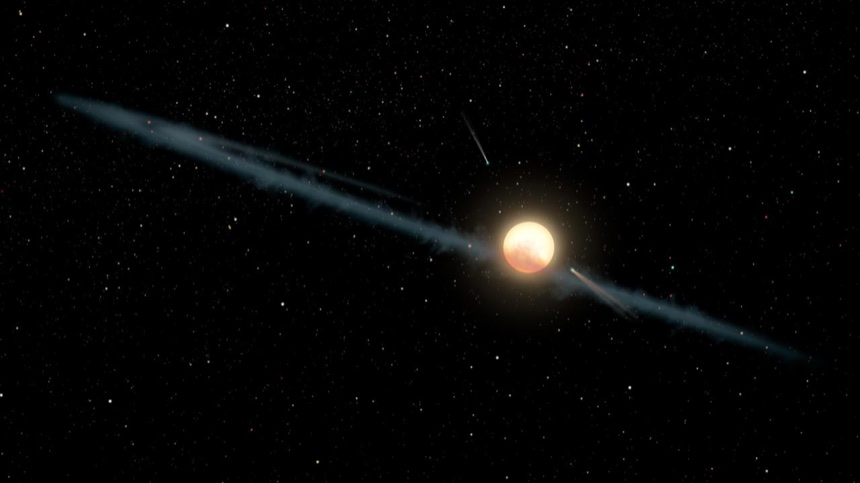
\includegraphics[width=0.78\textwidth,height=5.6cm,keepaspectratio]{../public/textures/nasa/parker.jpg}\\[3pt]
{\footnotesize\itshape\color{orbitarMuted} Imagine oficială NASA/JHUAPL: Sonda Parker Solar Probe zburând prin coroana solară incandescentă.}
\end{center}


\begin{tcolorbox}[orbitardata, title={\textbf{Repere esențiale: Parker Solar Probe}}]
\small
\begin{itemize}[leftmargin=1.4em, itemsep=2pt, topsep=2pt]
  \item \textbf{Clasificare și orbită:} Sondă Interplanetară \quad$\bullet$\quad \textbf{Distanță:} 0,250 UA ($\approx$ 37 milioane de kilometri)
  \item \textbf{Dimensiuni și masă:} anvergură de aproximativ 2 metri \quad$\bullet$\quad masă: Vehicul spațial artificial
  \item \textbf{Gravitație și regim termic:} Microgravitație / Imponderabilitate ($\approx 0\,g$) \quad$\bullet$\quad temperatură medie: +1.370 $^\circ$C
  \item \textbf{Ciclu orbital și rotație:} perioadă orbitală (an): 88 zile pământești \quad$\bullet$\quad rotație (zi): 24,00 ore (1,00 zile pământești) (elemente kepleriene: $a = 0,390$ UA, $e = 0,8800$, $i = 3,40^\circ$, $\Omega = 75,0^\circ$, $\omega = 15,0^\circ$)
  \item \textbf{Durata călătoriei de pe Pământ:} cu viteza luminii ($1c$): \emph{8 minute}; cu racheta ($50.000$ de kilometri pe oră): \emph{câteva luni}; cu avionul ($900$ de kilometri pe oră): \emph{18 ani}; cu mașina ($100$ de kilometri pe oră): \emph{160 de ani}.
  \item \textbf{Repere de scară și curiozitate:} Are în față un scut termic special, gros cât o carte, în spatele căruia instrumentele stau la o temperatură plăcută de cameră în timp ce afară sunt +1.400 $^\circ$C! Atinge viteza incredibilă de 690.000 de kilometri pe oră, viteză cu care ai ajunge de la București la Oradea în mai puțin de 3 secunde!
\end{itemize}
\end{tcolorbox}

\vspace{4pt}
\noindent\textbf{Prezentare generală și profil astrofizic.} Lansată în august 2018 și numită în onoarea astrofizicianului Eugene Parker (care a prezis existența vântului solar), sonda folosește 7 asistențe gravitaționale ale planetei Venus pentru a coborî periheliul până la aproximativ 6,1 milioane de kilometri de fotosfera solară. Parker Solar Probe este cea mai rapidă navă construită vreodată de oameni și singura care s-a apropiat atât de mult de Soare încât a zburat chiar prin atmosfera lui de foc! Are în față un scut termic special, gros cât o carte, în spatele căruia instrumentele stau la o temperatură plăcută de cameră în timp ce afară sunt +1.400 $^\circ$C!

\medskip
\noindent\textbf{Arhitectura tehnică și instrumentele științifice de la bord.} Din punct de vedere constructiv și ingineresc, vehiculul spațial reunește mai multe subsisteme și instrumente științifice de înaltă precizie, proiectate să funcționeze în condițiile extreme ale spațiului cosmic. În primul rând se remarcă \textbf{Scutul de protecție termică (Thermal Protection System)}, gros de 11,4 centimetri din compozit carbon-carbon și spumă de carbon, rezistă la temperaturi de 1.370 $^\circ$C. În strânsă legătură cu această componentă se află \textbf{Panouri solare răcite activ cu apă deionizată}, care se retrag în umbra scutului termic în timpul trecerilor apropiate pe lângă Soare. În completarea acestui ansamblu întâlnim \textbf{Instrumentele FIELDS, SWEAP, WISPR și IS$_\odot$IS}, care măsoară câmpurile magnetice, plasma coronală și fotografiaza structurile vântului solar.

\medskip
\noindent\textbf{Observații astronomice și istoricul explorării.} În 2021 a devenit prima navă care a traversat suprafața critică Alfvén, intrând oficial în atmosfera magnetică a Soarelui. Atinge viteza incredibilă de 690.000 de kilometri pe oră, viteză cu care ai ajunge de la București la Oradea în mai puțin de 3 secunde!

\vspace{6pt}
\begin{tcolorbox}[orbitarquiz, title={\textbf{Întrebare de verificare \#42: Parker Solar Probe}}]
\textbf{Ce record absolut deține sonda Parker Solar Probe?}
\begin{itemize}[leftmargin=2.2em, itemsep=2pt, topsep=4pt]
  \item[$\square$ \textbf{A.}] Cea mai grea rachetă
  \item[$\square$ \textbf{B.}] Cel mai rapid obiect construit vreodată de om (aproximativ 690.000 kilometri pe oră) și cel mai apropiat de Soare
  \item[$\square$ \textbf{C.}] Cea mai veche sondă
  \item[$\square$ \textbf{D.}] Singura sondă de pe Marte
\end{itemize}
\vspace{2pt}
{\footnotesize\color{orbitarMuted}\textbf{Răspuns corect:} \textbf{B} (Cel mai rapid obiect construit vreodată de om (aproximativ 690.000 kilometri pe oră) și cel mai apropiat de Soare). \emph{Atrăgând-o gravitația imensă a Soarelui la periheliu, Parker Solar Probe atinge aproximativ 191 kilometri pe secundă (690.000 kilometri pe oră).}}
\end{tcolorbox}
\clearpage


\section{Rosetta \& Philae}
\label{sec:body-rosetta}
\vspace{-4pt}
{\large\itshape\color{orbitarAccent} Misiunea europeană istorică ce a însoțit o cometă și a asolizat pe nucleul ei}\\[4pt]


\begin{center}
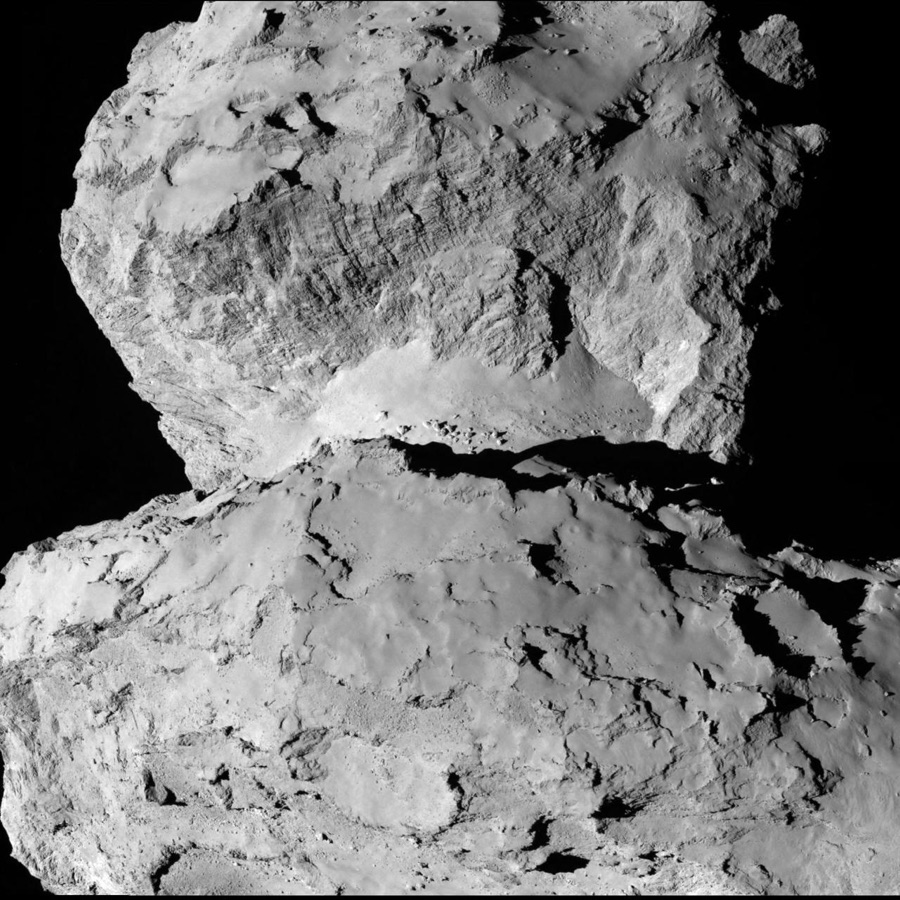
\includegraphics[width=0.78\textwidth,height=5.6cm,keepaspectratio]{../public/textures/nasa/rosetta.jpg}\\[3pt]
{\footnotesize\itshape\color{orbitarMuted} Fotografie oficială ESA/NASA (PIA18596): Nucleul bilobat al cometei 67P/Ciuriumov-Gherasimenko fotografiat de sonda Rosetta.}
\end{center}


\begin{tcolorbox}[orbitardata, title={\textbf{Repere esențiale: Rosetta \& Philae}}]
\small
\begin{itemize}[leftmargin=1.4em, itemsep=2pt, topsep=2pt]
  \item \textbf{Clasificare și orbită:} Sondă Interplanetară \quad$\bullet$\quad \textbf{Distanță:} 3,460 UA ($\approx$ 518 milioane de kilometri)
  \item \textbf{Dimensiuni și masă:} anvergură de aproximativ 2 metri \quad$\bullet$\quad masă: Vehicul spațial artificial
  \item \textbf{Gravitație și regim termic:} Microgravitație / Imponderabilitate ($\approx 0\,g$) \quad$\bullet$\quad temperatură medie: -70 $^\circ$C
  \item \textbf{Ciclu orbital și rotație:} perioadă orbitală (an): 2.352 zile ($\approx$ 6,44 ani pământești) \quad$\bullet$\quad rotație (zi): 12,40 ore (0,52 zile pământești) (elemente kepleriene: $a = 3,460$ UA, $e = 0,6400$, $i = 7,04^\circ$, $\Omega = 50,1^\circ$, $\omega = 12,8^\circ$)
  \item \textbf{Durata călătoriei de pe Pământ:} cu viteza luminii ($1c$): \emph{28 de minute}; cu racheta ($50.000$ de kilometri pe oră): \emph{10 ani (pe o traiectorie cu asistențe gravitaționale)}; cu avionul ($900$ de kilometri pe oră): \emph{50 de ani}; cu mașina ($100$ de kilometri pe oră): \emph{450 de ani}.
  \item \textbf{Repere de scară și curiozitate:} Cometa pe care a ajuns Rosetta are exact forma unei rățuște de baie din gheață și praf negru, lungă de 4 kilometri! Aripile solare ale sondei Rosetta erau lungi de 32 de metri, având lungimea unei balene albastre!
\end{itemize}
\end{tcolorbox}

\vspace{4pt}
\noindent\textbf{Prezentare generală și profil astrofizic.} Lansată de ESA în martie 2004, Rosetta a devenit în august 2014 prima sondă care a intrat pe orbita unei comete (67P/Ciuriumov-Gherasimenko), iar la 12 noiembrie 2014 modulul său Philae a realizat prima asolizare moale pe nucleul unei comete. Rosetta a fost sonda Agenției Spațiale Europene care a urmărit timp de 10 ani cometa Ciuriumov-Gherasimenko și a coborât pe ea micul robot laborator Philae! Cometa pe care a ajuns Rosetta are exact forma unei rățuște de baie din gheață și praf negru, lungă de 4 kilometri!

\medskip
\noindent\textbf{Arhitectura tehnică și instrumentele științifice de la bord.} Din punct de vedere constructiv și ingineresc, vehiculul spațial reunește mai multe subsisteme și instrumente științifice de înaltă precizie, proiectate să funcționeze în condițiile extreme ale spațiului cosmic. În primul rând se remarcă \textbf{Aripi solare de 64 metri pătrați cu celule LILT}, proiectate pentru intensitate luminoasă scăzută și temperaturi joase până la 5,2 UA de Soare. În strânsă legătură cu această componentă se află \textbf{Modulul de asolizare Philae (100 de kilograme)}, echipat cu harpoane, burghiu de eșantionare și 10 instrumente de analiză chimică și izotopică. În completarea acestui ansamblu întâlnim \textbf{Spectrometrul ROSINA și camera OSIRIS}, care au detectat aminoacidul glicină, fosfor și raportul deuteriu/hidrogen din apa cometară.

\medskip
\noindent\textbf{Observații astronomice și istoricul explorării.} Și-a încheiat misiunea la 30 septembrie 2016 coborând lent și așezându-se definitiv pe suprafața cometei 67P. Aripile solare ale sondei Rosetta erau lungi de 32 de metri, având lungimea unei balene albastre!

\vspace{6pt}
\begin{tcolorbox}[orbitarquiz, title={\textbf{Întrebare de verificare \#43: Rosetta \& Philae}}]
\textbf{Ce premieră mondială a realizat misiunea europeană Rosetta în anul 2014?}
\begin{itemize}[leftmargin=2.2em, itemsep=2pt, topsep=4pt]
  \item[$\square$ \textbf{A.}] A ajuns pe Pluto
  \item[$\square$ \textbf{B.}] A intrat pe orbita unei comete (67P) și a așezat robotul Philae pe suprafața ei
  \item[$\square$ \textbf{C.}] A adus roci de pe Marte
  \item[$\square$ \textbf{D.}] A fotografiat Soarele din interior
\end{itemize}
\vspace{2pt}
{\footnotesize\color{orbitarMuted}\textbf{Răspuns corect:} \textbf{B} (A intrat pe orbita unei comete (67P) și a așezat robotul Philae pe suprafața ei). \emph{Rosetta și modulul Philae au realizat prima orbitare și prima asolizare din istorie pe nucleul unei comete.}}
\end{tcolorbox}
\clearpage


\section{JUICE (Jupiter Icy Moons Explorer)}
\label{sec:body-juice}
\vspace{-4pt}
{\large\itshape\color{orbitarAccent} Exploratorul european al lunilor înghețate cu oceane ale lui Jupiter}\\[4pt]


\begin{center}
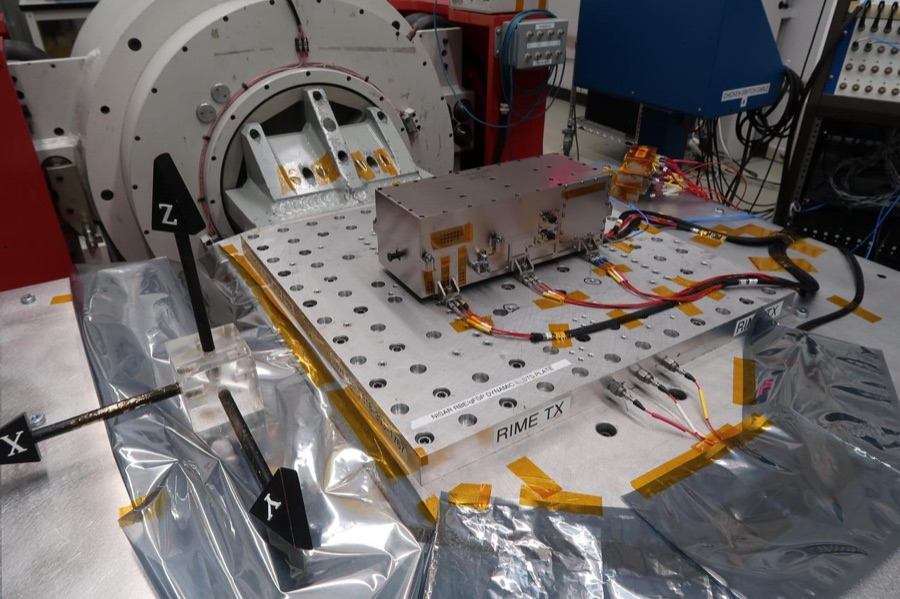
\includegraphics[width=0.78\textwidth,height=5.6cm,keepaspectratio]{../public/textures/nasa/juice.jpg}\\[3pt]
{\footnotesize\itshape\color{orbitarMuted} Fotografie oficială NASA/JPL/ESA (PIA24024): Sonda interplanetară europeană JUICE destinată studiului lunilor înghețate ale lui Jupiter.}
\end{center}


\begin{tcolorbox}[orbitardata, title={\textbf{Repere esențiale: JUICE (Jupiter Icy Moons Explorer)}}]
\small
\begin{itemize}[leftmargin=1.4em, itemsep=2pt, topsep=2pt]
  \item \textbf{Clasificare și orbită:} Sondă Interplanetară \quad$\bullet$\quad \textbf{Distanță:} 3,100 UA ($\approx$ 464 milioane de kilometri)
  \item \textbf{Dimensiuni și masă:} anvergură de aproximativ 2 metri \quad$\bullet$\quad masă: Vehicul spațial artificial
  \item \textbf{Gravitație și regim termic:} Microgravitație / Imponderabilitate ($\approx 0\,g$) \quad$\bullet$\quad temperatură medie: -150 $^\circ$C
  \item \textbf{Ciclu orbital și rotație:} perioadă orbitală (an): 1.850 zile ($\approx$ 5,07 ani pământești) \quad$\bullet$\quad rotație (zi): 24,00 ore (1,00 zile pământești) (elemente kepleriene: $a = 3,100$ UA, $e = 0,5200$, $i = 2,10^\circ$, $\Omega = 210,0^\circ$, $\omega = 60,0^\circ$)
  \item \textbf{Durata călătoriei de pe Pământ:} cu viteza luminii ($1c$): \emph{35 de minute}; cu racheta ($50.000$ de kilometri pe oră): \emph{8 ani (lansată în 2023, sosire la Jupiter în 2031)}; cu avionul ($900$ de kilometri pe oră): \emph{80 de ani}; cu mașina ($100$ de kilometri pe oră): \emph{717 ani}.
  \item \textbf{Repere de scară și curiozitate:} Cele două aripi solare ale sale, în formă de cruce, sunt mari cât un teren de baschet! Pe fuselajul sondei JUICE este gravat un desen realizat de o fetiță de 10 ani, ales dintr-un concurs la care au participat mii de copii!
\end{itemize}
\end{tcolorbox}

\vspace{4pt}
\noindent\textbf{Prezentare generală și profil astrofizic.} Lansată la 14 aprilie 2023 cu o rachetă Ariane 5, misiunea de clasă mare a ESA (JUICE) va ajunge în sistemul jovian în iulie 2031, va efectua 35 de survoluri ale lunilor Europa, Callisto și Ganymede, iar în 2034 va deveni prima sondă care orbitează o lună a altei planete (Ganymede). JUICE este sonda Agenției Spațiale Europene aflată în drum spre Jupiter pentru a cerceta oceanele ascunse sub gheață de pe lunile Europa, Callisto și Ganymede! Cele două aripi solare ale sale, în formă de cruce, sunt mari cât un teren de baschet!

\medskip
\noindent\textbf{Arhitectura tehnică și instrumentele științifice de la bord.} Din punct de vedere constructiv și ingineresc, vehiculul spațial reunește mai multe subsisteme și instrumente științifice de înaltă precizie, proiectate să funcționeze în condițiile extreme ale spațiului cosmic. În primul rând se remarcă \textbf{Panouri solare în formă de cruce (85 metri pătrați)}, cel mai mare sistem fotovoltaic trimis vreodată către Sistemul Solar exterior (unde lumina solară este de 25 de ori mai slabă). În strânsă legătură cu această componentă se află \textbf{Radarul de penetrare a gheții RIME (antena de 16 metri)}, care poate \guillemotleft{}vedea\guillemotright{} până la 9 kilometri adâncime prin crusta de gheață a lunilor joviane. În completarea acestui ansamblu întâlnim \textbf{Magnetometrul J-MAG și altimetrul laser GALA}, care vor măsura adâncimea și salinitatea oceanelor subterane de pe Ganymede, Europa și Callisto.

\medskip
\noindent\textbf{Observații astronomice și istoricul explorării.} În august 2024 a realizat prima manevră dublă din istorie de asistență gravitațională Lună--Pământ (LEGA). Pe fuselajul sondei JUICE este gravat un desen realizat de o fetiță de 10 ani, ales dintr-un concurs la care au participat mii de copii!

\vspace{6pt}
\begin{tcolorbox}[orbitarquiz, title={\textbf{Întrebare de verificare \#44: JUICE (Jupiter Icy Moons Explorer)}}]
\textbf{În jurul cărui satelit natural va intra pe orbită sonda europeană JUICE în anul 2034?}
\begin{itemize}[leftmargin=2.2em, itemsep=2pt, topsep=4pt]
  \item[$\square$ \textbf{A.}] Luna Pământului
  \item[$\square$ \textbf{B.}] Ganymede (cel mai mare satelit al lui Jupiter)
  \item[$\square$ \textbf{C.}] Titan
  \item[$\square$ \textbf{D.}] Io
\end{itemize}
\vspace{2pt}
{\footnotesize\color{orbitarMuted}\textbf{Răspuns corect:} \textbf{B} (Ganymede (cel mai mare satelit al lui Jupiter)). \emph{JUICE va deveni prima sondă din istorie care va intra pe orbită în jurul unui satelit al altei planete: Ganymede.}}
\end{tcolorbox}
\clearpage


\section{Perseverance \& Ingenuity}
\label{sec:body-perseverance}
\vspace{-4pt}
{\large\itshape\color{orbitarAccent} Laboratorul astrobiologic pe roți și primul elicopter care a zburat pe Marte}\\[4pt]


\begin{center}
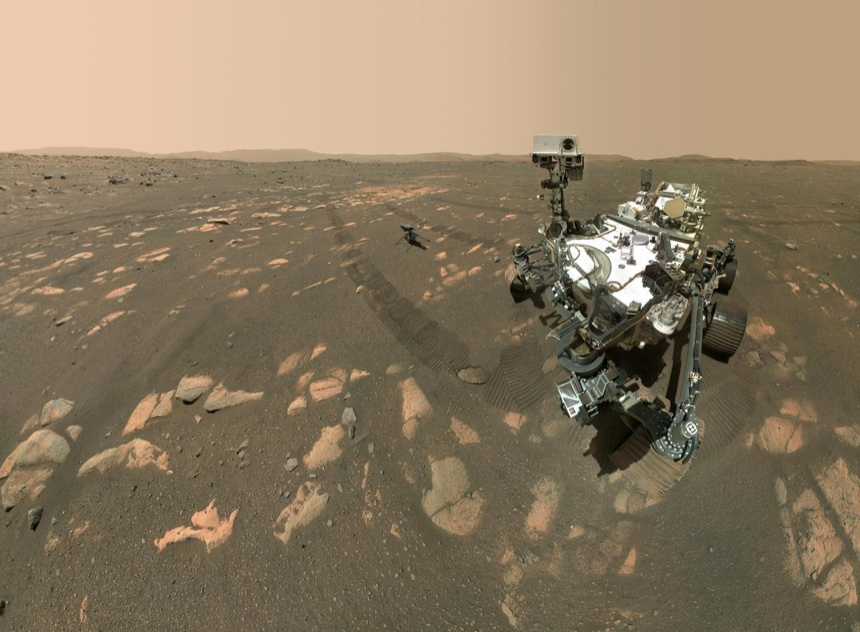
\includegraphics[width=0.78\textwidth,height=5.6cm,keepaspectratio]{../public/textures/nasa/perseverance.jpg}\\[3pt]
{\footnotesize\itshape\color{orbitarMuted} Fotografie reală NASA/JPL-Caltech (PIA24542): Roverul Perseverance alături de elicopterul Ingenuity în Craterul Jezero de pe Marte.}
\end{center}


\begin{tcolorbox}[orbitardata, title={\textbf{Repere esențiale: Perseverance \& Ingenuity}}]
\small
\begin{itemize}[leftmargin=1.4em, itemsep=2pt, topsep=2pt]
  \item \textbf{Clasificare și orbită:} Rover Planetar (orbitează în jurul: \textbf{Marte}) \quad$\bullet$\quad \textbf{Distanță:} 1,524 UA ($\approx$ 228 milioane de kilometri)
  \item \textbf{Dimensiuni și masă:} anvergură de aproximativ 2 metri \quad$\bullet$\quad masă: Vehicul spațial artificial
  \item \textbf{Gravitație și regim termic:} 0,380 $\times g_\oplus$ (3,73 m/s$^2$) \quad$\bullet$\quad temperatură medie: -63 $^\circ$C
  \item \textbf{Ciclu orbital și rotație:} perioadă orbitală (an): 686,98 zile ($\approx$ 1,88 ani pământești) \quad$\bullet$\quad rotație (zi): 24,62 ore (1,03 zile pământești)
  \item \textbf{Durata călătoriei de pe Pământ:} cu viteza luminii ($1c$): \emph{între 3 și 22 de minute}; cu racheta ($50.000$ de kilometri pe oră): \emph{7 luni (lansat în iulie 2020, amartizat în februarie 2021)}; cu avionul ($900$ de kilometri pe oră): \emph{7 ani}; cu mașina ($100$ de kilometri pe oră): \emph{62 de ani}.
  \item \textbf{Repere de scară și curiozitate:} Roverul este mare cât o mașină de teren, iar elicopterul Ingenuity cântărește doar 1,8 kilograme, cam cât o cutie mare de lapte! Ingenuity a fost primul aparat din istorie care a zburat pe o altă planetă, reușind 72 de zboruri în aerul subțire al lui Marte!
\end{itemize}
\end{tcolorbox}

\vspace{4pt}
\noindent\textbf{Prezentare generală și profil astrofizic.} Amartizat la 18 februarie 2021 în craterul Jezero (delta unui râu antic marțian), Perseverance caută biosemnături fosile, colectează carote de rocă în tuburi sigilate pentru viitoarea aducere pe Pământ și a demonstrat producerea de oxigen din atmosfera marțiană. Perseverance (\guillemotleft{}Percy\guillemotright{}) este un robot explorator pe 6 roți care caută urme de viață străveche în craterul Jezero de pe Marte, însoțit de micul elicopter Ingenuity (\guillemotleft{}Ginny\guillemotright{})! Roverul este mare cât o mașină de teren, iar elicopterul Ingenuity cântărește doar 1,8 kilograme, cam cât o cutie mare de lapte!

\medskip
\noindent\textbf{Arhitectura tehnică și instrumentele științifice de la bord.} Din punct de vedere constructiv și ingineresc, vehiculul spațial reunește mai multe subsisteme și instrumente științifice de înaltă precizie, proiectate să funcționeze în condițiile extreme ale spațiului cosmic. În primul rând se remarcă \textbf{Catargul cu SuperCam și Mastcam-Z}, camere panoramice cu zoom și un laser care vaporizează rocile de la 7 metri distanță pentru a le analiza compoziția. În strânsă legătură cu această componentă se află \textbf{Experimentul MOXIE}, care a produs cu succes oxigen respirabil direct din dioxidul de carbon (CO$_2$) al atmosferei marțiene. În completarea acestui ansamblu întâlnim \textbf{Elicopterul coaxial Ingenuity}, elice din fibră de carbon care se rotesc cu 2.400 rpm pentru a genera portanță în atmosfera marțiană cu densitate de doar 1\%.

\medskip
\noindent\textbf{Observații astronomice și istoricul explorării.} Coborât pe Marte prin spectaculoasa manevră \guillemotleft{}Sky Crane\guillemotright{} (macara zburătoare cu rachete); Ingenuity a zburat de 72 de ori între 2021 și 2024. Ingenuity a fost primul aparat din istorie care a zburat pe o altă planetă, reușind 72 de zboruri în aerul subțire al lui Marte!

\vspace{6pt}
\begin{tcolorbox}[orbitarquiz, title={\textbf{Întrebare de verificare \#45: Perseverance \& Ingenuity}}]
\textbf{Ce a demonstrat în premieră instrumentul MOXIE de la bordul roverului Perseverance?}
\begin{itemize}[leftmargin=2.2em, itemsep=2pt, topsep=4pt]
  \item[$\square$ \textbf{A.}] Că pe Marte plouă cu apă
  \item[$\square$ \textbf{B.}] Că se poate produce oxigen pur din atmosfera de dioxid de carbon a lui Marte
  \item[$\square$ \textbf{C.}] Că Marte are câmp magnetic puternic
  \item[$\square$ \textbf{D.}] Că există plante verzi
\end{itemize}
\vspace{2pt}
{\footnotesize\color{orbitarMuted}\textbf{Răspuns corect:} \textbf{B} (Că se poate produce oxigen pur din atmosfera de dioxid de carbon a lui Marte). \emph{MOXIE a extras oxigen din CO$_2$-ul atmosferic marțian, o tehnologie esențială pentru viitorii astronauți (pentru respirație și combustibil de rachetă).}}
\end{tcolorbox}
\clearpage


\section{Curiosity (Mars Science Laboratory)}
\label{sec:body-curiosity}
\vspace{-4pt}
{\large\itshape\color{orbitarAccent} Roverul veteran care urcă pe Muntele Sharp din craterul Gale de pe Marte}\\[4pt]


\begin{center}
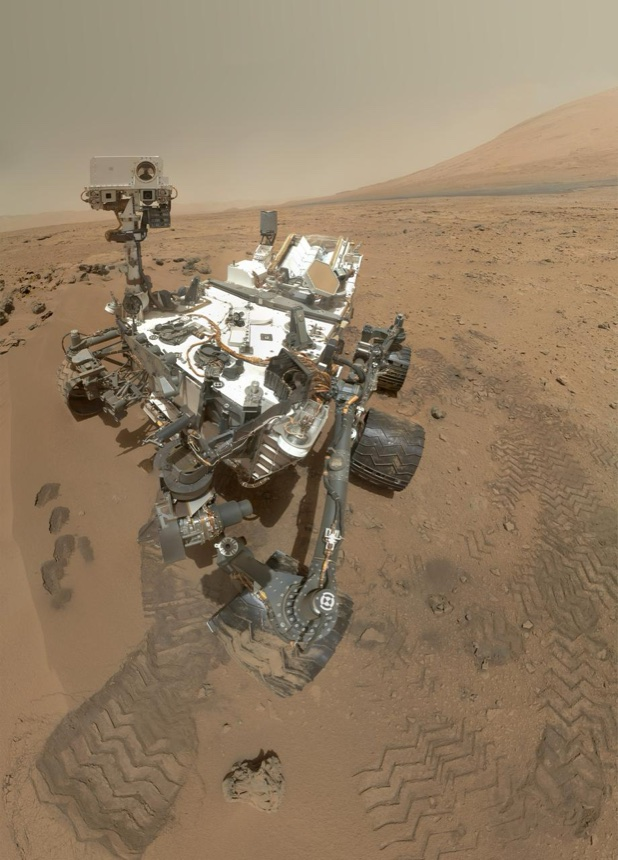
\includegraphics[width=0.78\textwidth,height=5.6cm,keepaspectratio]{../public/textures/nasa/curiosity.jpg}\\[3pt]
{\footnotesize\itshape\color{orbitarMuted} Autoportret real NASA/JPL-Caltech (PIA16239): Roverul Curiosity (MSL) pe solul Craterului Gale de pe Marte.}
\end{center}


\begin{tcolorbox}[orbitardata, title={\textbf{Repere esențiale: Curiosity (Mars Science Laboratory)}}]
\small
\begin{itemize}[leftmargin=1.4em, itemsep=2pt, topsep=2pt]
  \item \textbf{Clasificare și orbită:} Rover Planetar (orbitează în jurul: \textbf{Marte}) \quad$\bullet$\quad \textbf{Distanță:} 1,524 UA ($\approx$ 228 milioane de kilometri)
  \item \textbf{Dimensiuni și masă:} anvergură de aproximativ 2 metri \quad$\bullet$\quad masă: Vehicul spațial artificial
  \item \textbf{Gravitație și regim termic:} 0,380 $\times g_\oplus$ (3,73 m/s$^2$) \quad$\bullet$\quad temperatură medie: -63 $^\circ$C
  \item \textbf{Ciclu orbital și rotație:} perioadă orbitală (an): 686,98 zile ($\approx$ 1,88 ani pământești) \quad$\bullet$\quad rotație (zi): 24,62 ore (1,03 zile pământești)
  \item \textbf{Durata călătoriei de pe Pământ:} cu viteza luminii ($1c$): \emph{între 3 și 22 de minute}; cu racheta ($50.000$ de kilometri pe oră): \emph{8 luni și jumătate (2011--2012)}; cu avionul ($900$ de kilometri pe oră): \emph{7 ani}; cu mașina ($100$ de kilometri pe oră): \emph{62 de ani}.
  \item \textbf{Repere de scară și curiozitate:} Curiosity are un \guillemotleft{}cap\guillemotright{} cu 17 camere foto și un braț robotic lung de 2 metri cu care găurește pietrele marțiene! Roțile lui Curiosity au găuri speciale care lasă pe nisipul de pe Marte urme în codul Morse cu literele \guillemotleft{}J P L\guillemotright{} (laboratorul care l-a construit)!
\end{itemize}
\end{tcolorbox}

\vspace{4pt}
\noindent\textbf{Prezentare generală și profil astrofizic.} Amartizat la 6 august 2012 în craterul Gale, Curiosity (900 de kilograme, alimentat nuclear prin RTG) urcă treptat pe versanții muntelui Aeolis Mons (Mount Sharp, 5,5 kilometri înălțime), citind în straturile sedimentare tranziția lui Marte de la o lume umedă la un deșert rece. Curiosity este laboratorul chimic pe roți care explorează Marte încă din anul 2012! El a demonstrat că pe Marte au existat lacuri cu apă dulce în care ar fi putut trăi microbi. Curiosity are un \guillemotleft{}cap\guillemotright{} cu 17 camere foto și un braț robotic lung de 2 metri cu care găurește pietrele marțiene!

\medskip
\noindent\textbf{Arhitectura tehnică și instrumentele științifice de la bord.} Din punct de vedere constructiv și ingineresc, vehiculul spațial reunește mai multe subsisteme și instrumente științifice de înaltă precizie, proiectate să funcționeze în condițiile extreme ale spațiului cosmic. În primul rând se remarcă \textbf{Laboratorul intern SAM (Sample Analysis at Mars)}, spectrometru de masă și cromatograf cu gaz care a identificat molecule organice complexe în argilele marțiene. În strânsă legătură cu această componentă se află \textbf{Instrumentul cu laser ChemCam și difractometrul CheMin}, care identifică mineralele formate în prezența apei cu pH neutru. În completarea acestui ansamblu întâlnim \textbf{Suspensia Rocker-Bogie cu 6 roți motoare}, care permite roverului să treacă peste obstacole de două ori mai mari decât diametrul roților fără să se răstoarne.

\medskip
\noindent\textbf{Observații astronomice și istoricul explorării.} A parcurs peste 32 de kilometri pe Marte în mai mult de 4.300 de zile marțiene (soli), fiind încă activ. Roțile lui Curiosity au găuri speciale care lasă pe nisipul de pe Marte urme în codul Morse cu literele \guillemotleft{}J P L\guillemotright{} (laboratorul care l-a construit)!

\vspace{6pt}
\begin{tcolorbox}[orbitarquiz, title={\textbf{Întrebare de verificare \#46: Curiosity (Mars Science Laboratory)}}]
\textbf{Ce descoperire fundamentală a făcut roverul Curiosity în craterul Gale de pe Marte?}
\begin{itemize}[leftmargin=2.2em, itemsep=2pt, topsep=4pt]
  \item[$\square$ \textbf{A.}] Că Marte nu a avut niciodată apă
  \item[$\square$ \textbf{B.}] Că în trecutul îndepărtat al lui Marte au existat lacuri și râuri de apă lichidă cu condiții prielnice vieții microbiene
  \item[$\square$ \textbf{C.}] Că solul este din aur pur
  \item[$\square$ \textbf{D.}] Că Marte are inele
\end{itemize}
\vspace{2pt}
{\footnotesize\color{orbitarMuted}\textbf{Răspuns corect:} \textbf{B} (Că în trecutul îndepărtat al lui Marte au existat lacuri și râuri de apă lichidă cu condiții prielnice vieții microbiene). \emph{Analizând pietrișul rotunjit de apă și argilele din craterul Gale, Curiosity a demonstrat că Marte a găzduit lacuri străvechi de apă potabilă.}}
\end{tcolorbox}
\clearpage

